% Review Christian Stary January 2020

\chapter{Implementation of Subject-Oriented Models}

Subject oriented models address the internal aspects and structures of a system. They are essentially models of the internal structure of a system and cover organizational and technical aspects. When implementing the models, it is now necessary to establish the relationship between the process model and the available resources. Figure \ref{fig:Implementation-steps} shows the individual steps from a process model to the executable process instance.

\begin{figure}[h]
	\centering
	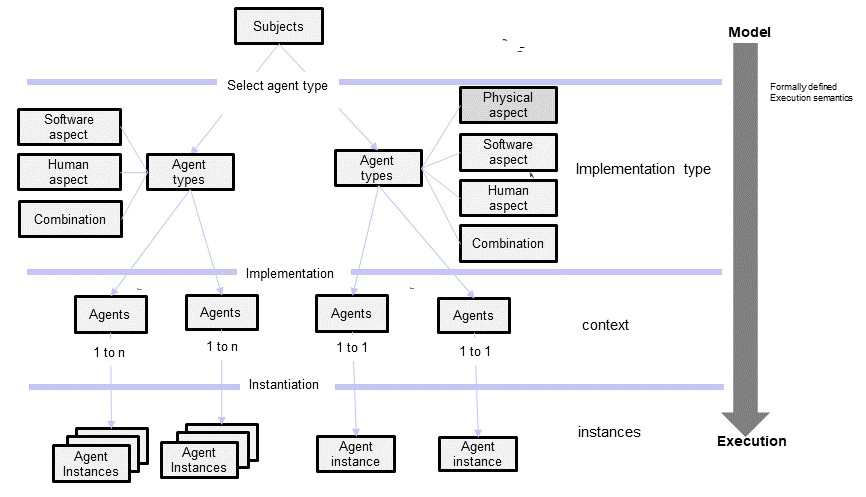
\includegraphics[width=0.9\linewidth]{Figures/Implementation/Implementation-steps.jpg}
	\caption[Implementation steps]{Implementation steps}
	\label{fig:Implementation-steps}
\end{figure}
 
In a system model, the actors, the actions, their sequences and the objects manipulated by the actions are described. Actions (activities) can be performed by humans, software systems, physical systems or a combination of these basic types of actors. We call them the task holders. For example, a software system can automatically perform the "tax rate calculation" action, while a person uses a software program to perform the "order entry" activity. The person enters the order data via a screen mask. The software checks the entered data for plausibility and saves it. However, activities can also be carried out purely manually, for example when a warehouse worker receives a picking order on paper, executes it, marks it as executed on the order form and returns it to the warehouse manager.\\ 
When creating a system model, it is often not yet known which types of actors execute which actions. Therefore, it can be useful to abstract from said CS: said?? the?  model when starting to describe processes by introducing abstract actors. A modeling language should allow the use of such abstractions. This means that when defining the process logic, no assertion should have to be made about what type of actor is realized. In S-BPM, the subjects represent abstract actors. \\
In the description of the control logic of a process, the individual activities are also described independently of their implementation. For example, for the action "create a picking order" it is not specified whether a human actor fills in a paper form or a screen mask, or whether a software system generates this form automatically. Thus, with activities the means by which something happens is not described, but rather only what happens.\\ 
The means are of course related to the implementation type of the actor. As soon as it has been defined which types of actors are assigned to the individual actions, the manner of realization of an activity has also been defined. In addition, the logical or physical object on which an action is executed also needs to be determined. Logical objects are data structures whose data is manipulated by activities. Paper forms represent a mixture between logical and physical objects, while a workpiece on which the "deburring" action takes place is a purely physical object. Therefore, there is a close relationship between the type of task holder, the actions and the associated objects actors manipulate or use when performing actions.\\
A system model can be used in different areas. The process logic is applied unchanged in the respective areas. However, it may be necessary to implement the individual actors and actions differently. Thus, in one environment certain actions could be performed by humans and in another the same actions could be performed by software systems. In the following, we refer to such different environments of use for a system model as context. Hence, for a process model, varying contexts can exist, in which there are different realization types for actors and actions.\\ 
In Subject Oriented Modeling, actors are not assigned to individual activities, but rather the actor type is assigned to an entire subject. This assignment is not part of the process logic, but in the most simple way it is done instead for each process in a separate two-column table. The left column contains the subject name and the right column the implementation type. If there are several contexts for a model, a separate assignment table is created for each of them.
The assignment of the implementation type forms the transition from the system logic and its implementation. Subsequently, it has to be defined which persons, software systems and physical systems represent the actors and how the individual actions are concretely realized. These aspects are described in detail in the following subsections.

\section{People and organizations}


\section{Physical infrastructure}

\section{IT-Systems and Software}

